\documentclass[11pt,a4paper]{article}
\usepackage[utf8]{inputenc}
\usepackage{amsmath}
\usepackage{amsfonts}
\usepackage{amssymb}
\usepackage{graphicx}
\usepackage{mathtools}
\usepackage[backend=bibtex,style=verbose-ibid]{biblatex}
\addbibresource{citations.bib}


\usepackage{listings}
\usepackage{color}
\definecolor{dkgreen}{rgb}{0,0.6,0}
\definecolor{gray}{rgb}{0.5,0.5,0.5}
\definecolor{mauve}{rgb}{0.58,0,0.82}

\lstset{frame=tb,
  language=Python,
  aboveskip=3mm,
  belowskip=3mm,
  showstringspaces=false,
  columns=flexible,
  basicstyle={\small\ttfamily},
  numbers=none,
  numberstyle=\tiny\color{gray},
  keywordstyle=\color{blue},
  commentstyle=\color{dkgreen},
  stringstyle=\color{mauve},
  breaklines=true,
  breakatwhitespace=true,
  tabsize=3
}


\newcommand{\inv}{^{\raisebox{.2ex}{$\scriptscriptstyle-1$}}}
\newcommand{\qed}{\hfill $\blacksquare$}
\newcommand{\reals}{\mathbb{R}}
\newcommand{\complexes}{\mathbb{C}}
\newcommand{\field}{\mathbb{F}}
\author{Jacob Bruner}
\title{IB Extended Essay}
\date{\today}

\begin{document}
\maketitle
\tableofcontents

\pagebreak

\iffalse
############
heres an example of a code block
\begin{lstlisting}
        def intervalValues(z, n):
            return output # return the sequence of values
\end{lstlisting}

heres an example of an image
\begin{figure}[h]
\begin{center}
\includegraphics[scale=.37]{onefifteen} 
\caption{Sequences Generated by n = 1-15 on Argand Diagram}
\end{center}
\end{figure}
############
\fi

\section{Introduction and Aim}
\subsection{Motivating Problem}
It's undeniable that our modern-day world is reliant on cryptography. Every time a phone sends a text, a browser connects to a server, an email gets sent off, a monetary transaction is made, and much much more, our devices are, unbeknownst to us, performing many hundreds of math operations to ensure our data are 'encrypted.' But what does 'encryption' mean? Let's introduce some definitions. ‘Encryption’ is the process of disguising a message to be, loosely speaking, hidden to all but the intended recipient. This is the process of converting a ‘plaintext’ message into a jumbled ‘ciphertext’, which can be readily shared without risk of the sensitive message leaking. Converting a plaintext message (typically a string/list of characters) into a ciphertext is known as an ‘enciphering’ or ‘encrypting’ transformation. Likewise the reverse operation of recovering the plaintext message from a ciphertext is known as the \textit{deciphering transformation.}\autocite[54]{koblitz} If we denote the plain and cyphertext $\mathcal{P}$ and $\mathcal{C}$ respectively and the enciphering map $f$ and its inverse $f\inv$ we obtain the following diagram:

$$ \mathcal{P} \overset{f}\longrightarrow \mathcal{C} \overset{f\inv}\longrightarrow \mathcal{P} $$

The most common formulation for this kind of cryptosystem would be that the two transacting parties agree upon the parameters for the map $f$ in secret beforehand. Common examples include the 'Caeser Cipher' (supposedly invented by \textit{the} Julius Caeser), where $f$ is a shift operation that maps each letter to a new one a number of places ahead. We start encoding each letter as a number from 0, which is A, to 25, which is Z. Of course this depends on what alphabet one uses, if one chooses to include spaces etc. We can represent the operation that takes a letter and maps it $n$ places ahead with addition. Importantly, this operation must 'wrap around' back to zero if you try to exceed 'z' in the alphabet. This process, known as \textit{'modular arithmetic'}, is like circling a clock, where after reaching twelve, the hour hand wrap back around to 1, but we start from 0 instead of 1. So, in our case, shifting 'z' by 3 letters looks like so: $25 + 1 \bmod 26 \equiv 0$, which reads "25 plus 1 \textit{is congruent to} 0 \textit{modulo} (or \textit{mod}) 26". With this in mind, we obtain for each letter $p \in \mathcal{P}$:

\[
f(p) = p + n \bmod 26
\]

% I could maybe talk about affine cryptosystems here if I need more words.
% I could also show the linear algebra point of view

Representing a shifting of each letter in the plaintext by $n$ places in the alphabet. Now clearly this isn't a very sophisticated cryptographic scheme. For instance, performing a frequency analysis and comparing the most commonly occurring letters to that of the English alphabet can easily break these sorts of schemes, known as 'substitution ciphers.' Modern schemes typically employ more resistant techniques such that changing one letter of plaintext often yields a completely different ciphertext.
  For instance, AES encryption, part of the modern web standard, is an example of a block substitution cypher. At a high level, it combines techniques similar to our Caesar Cipher with certain affine transformations (which can be thought of as an additional scaling action in combination with our translation) performed on blocks of plaintext. It's certainly more complicated than that, but essentially boils down to our system plus some bells and whistles to make it resistant to cryptanalysis, like permutations, combinations, text look-up-tables and more. In general, this type of encryption where there's a predetermined shared secret is well-studied, often bearing the name 'symmetric-key encryption,' to emphasize that the private keys are known beforehand. For instance, Claude Shannon (often called the father of cryptography) mathematically proved that the 'one-time-pad' encryption technique was unbreakable. His findings showed that if a random-generated key is at least as long as the plaintext, performing modular addition (i.e., wrapping around so as to not exceed the alphabet) on each letter by the private key yields a ciphertext that is uncrackable.\autocite{claude} Although modern systems seek smaller key sizes for performance reasons, this worst-case scenario should demonstrate the strength of symmetric-key algorithms in general. The 'one-time-pad' gets its name from its use in WWII when the KGB would distribute palm-sized pads with these one-time-keys and a table to ease in conversion. Such pads were often made of flammable materials to be burned with no trace.\autocite{lewand} 
  
\begin{figure}[h]
\begin{center}
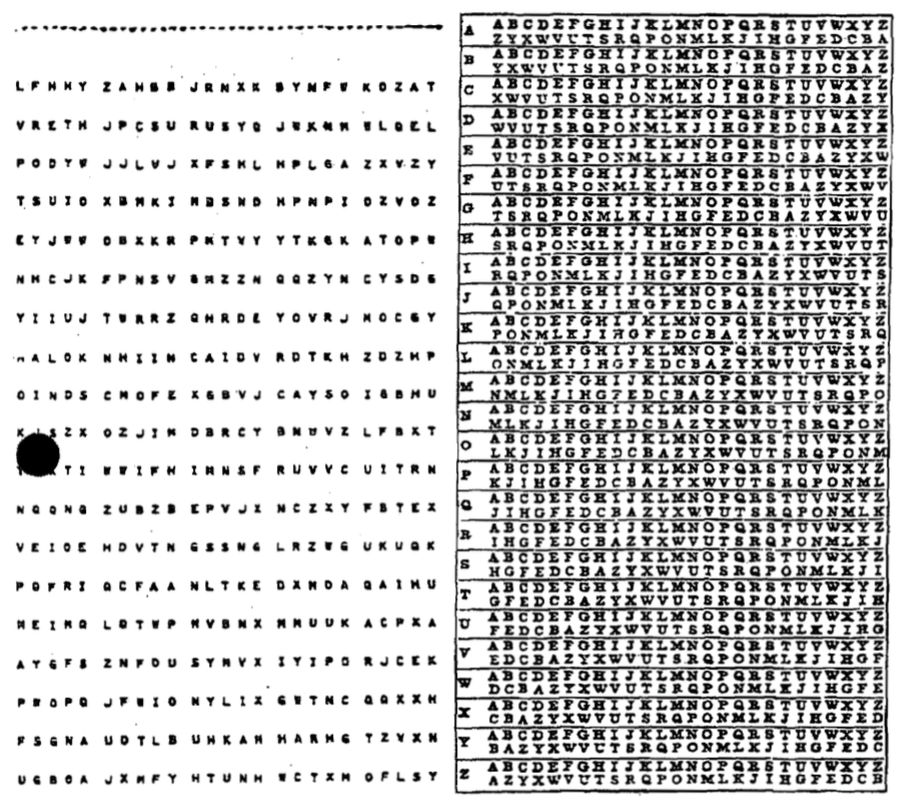
\includegraphics[scale=.29]{images/diana} 
\caption{Format of a one-time-pad used by the NSA\autocite{diana}}
\end{center}
\end{figure}
  

\subsection{The 'Public-Key' Paradox}

In the modern world, it's impractical to require that every shared secret be determined ahead of time. If a user wants to connect to a twitter server over a secure connection, how could symmetric-key encryption be employed? More generally, if two computers want to establish a connection for the first time, is there any way they could do so in an encrypted matter? The intuitive answer might be no, since how could you pass (or otherwise determine) a shared secret without any man-in-the-middle being able to obtain that same key. But this defys the ubiquity of encryption on the internet—every time I connect to a unfamiliar website, I still see a padlock on my browser. How can this be?

Consider the intuitive fact that some operations are more difficult to do in reverse than fowards—certain 'one-way functions.' For instance, if I mixed two different-colored paints together and asked whether you, \textit{a priori}, could deduce the two initial colors given the end result, would you be able to? Although its quite easy to check whether any two colors combine to match the end result, there isn't an easy operation that takes the end result and returns the initial colors. This happens to be true for a number of operations. 

\section{What is 'Public-Key' Cryptography}
"In applied contexts, the terms "easy" and "hard" are usually interpreted relative to some specific computing entity; typically "cheap enough for the legitimate users" and "prohibitively expensive for any malicious agents"."

The first protocol developed to address this motivating problem was RSA encryption. Leveraging intuitive properties of numbers, RSA establishes our idea of ‘one-way operations’ using simple multiplication of large, highly prime (minimal divisors), numbers. 

\section{How can we formalize this: An Introduction to Groups}
Group theory is the study of symmetry. The set of symmetries on an object correspond to a group, and every group corresponds to a set of symmetries.
\footnote{This is rigorously true if we consider the set of all automorphisms of an object (viz. the set of all bijective maps from and to itself), this forms a group under function composition with the inverses being the inverse maps and the identity being the identity "do nothing" map, so this perspective is justified.} % hmm
Now to unpack what this means, it might be helpful to expand our definitions of symmetry. The easiest examples are geometric symmetry. If we consider the set of all ways to leave a square unchanged by rotating or reflecting it, we obtain the 'Dihedral group of order 8,' denoted $\mathrm{D}_8$. More generally, the group of symmetries of an n-gon form the Dihedral group of order 2n, $\mathrm{D}_{2n}$. (Order, here, refers to the number of elements of the group, or the cardinality/size of the underlying set.)\footnote{The 'order' of an element also refers to the order/size of the subgroup generated by that element. Also, a group's order is allowed to be infinite.} Group theory allows us to categorize the 'extent' of these symmetries as well. For instance, the group of all symmetries on a circle is, intuitively, much larger than that of the rectangle. In fact, this circle group, denoted $\mathbb{T}$, is an especially important one in many respects, for instance establishing a certain duality between time and frequency, behaving as a topological space, and constituting a major part of the Standard Model of Physics.
  Now this interpretation of 'symmetry' is biased toward a very geometric perspective. If we want to broaden the horizons of group theory, we need to consider symmetries on objects like a law or principle, a mathematical equation, a structural rule, etc. In this interpretation, symmetry becomes a much deeper concept. For instance, our circle group above, $\mathbb{T}$, can also be represented as the set of all complex numbers with magnitude 1 under multiplication. 
\[
\mathbb{T} = ( \lbrace z \in \complexes \bigm| |z| = 1 \rbrace , \times )
\]
  Before I outright state the conditions that an object fits to be a group (the text-book definition), it might be helpful to see this type of thinking in action in the real-world. If we consider, as before, the 'law' or 'rule' that \textit{justice is impartial}, what we're essentially saying is that "the verdict of a court case is independent of the qualities of the people involved, as in, permuting the qualities of the people involved has no effect on the outcome." Mathematically, this would correspond to invarience under a certain group action, where the group action is the one that does the permuting. This perspective of indistinguishably does hint at Group theory's widespread use in cryptography. In essence, we're saying "one cannot \textit{a priori} give a property that holds for one instance and not another."
  To see where the textbook definition of a Group arises, we must first restrict the kinds of 'symmetries' we are looking for. Given a thing to be invariant and the type of transformations we're allowing, we can derive the group axioms like so: If we have two transformations $T_1, T_2$ that leave our object invariant we can see that their composition $T_1 \circ T_2$ must also leave the object invariant (composition referring to applying $T_2$ then applying $T_1$). Under this composition of transformations, one key property arises: \textit{associativity}. It might be hard to see at first glance, but function composition is always associative: the order in which you evaluate functions has no effect on the result. This means we can drop parenthesis without any ambiguity, since $T_1 \circ (T_2 \circ T_3) = (T_1 \circ T_2) \circ T_3 = T_1 \circ T_2 \circ T_2$. This can be seen diagrammatically, for maps $f, g, h$ below:
\begin{figure}[h]
\begin{center}
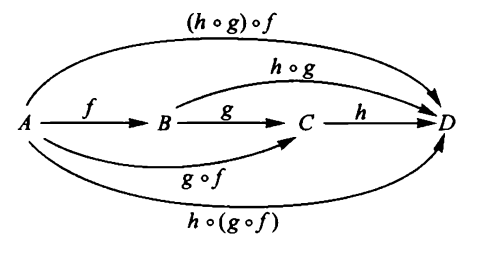
\includegraphics[scale=.4]{images/associativitydiagram} 
\end{center}
\end{figure}
Beyond associativity, another requirement is the "do nothing" map. At first seeming quite useless, it is the keystone of any group—the fundamental symmetry, if you will. This element is called the \textit{identity element} or the \textit{identity map}. The last criterion for a group is that of inverses. In a sense, this requirement that every map has an inverse map boils down to an interpretation that, in order to be a 'true' symmetry, it must be invertible. This should make sense, since, for example, if we had a map that 'forgot' some properties of an object, there wouldn't be an inverse map because this 'forgetful map' wouldn't be a bijection (one-to-one and onto). With that in mind, if one \textit{doesn't} restrict themselves to invertibility, we get another algebraic strucutre called a 'Monoid.' But the study of these are much more unwieldy and untame than that of groups, so this is a reasonable restriction.

\subsection*{The Definition of a Group}
  A group is a set $G$, equipped with a binary operation mapping two elements to another of the form $\ast:\ G \ast G \to G$ such that the following conditions hold:\autocite[16]{saracino}
\\\textbf{Associativity}
\\$\text{For all } a,b,c \in G,\ a\ast(b \ast c) = (a\ast b) \ast c$
\\\textbf{Identity}
\\$\text{There exists an element } e \in G \text{ such that } a \ast e = e \ast a = a \ \forall a \in G$
\\\textbf{Inverse}
\\$\text{Each element } x \in G \text{ has a unique inverse } x\inv \in G \text{ such that } x \ast x\inv = x\inv \ast x = e$


In our case, this set consisted of symmetry-preserving transformations on an object where the binary operation was function composition. It's worth mentioning that this axiomatic definition of a group was invented some 100 years after mathematicians began to study groups. It is for this reason that the 'symmetry' understanding of a group can often be more applicable to the answer "why study groups at all?". Under this axiomatic definition of a group, we can see a few glaring examples. For instance, the integers form a group under addition $(\mathbb{Z}, +)$. It's worth verifying for yourself that these do fit the definition of a group. Our identity element is 0, since $0 + a = a + 0 = a$ for all $a \in \mathbb{Z}$.
By forgoing the need to study a group's representation on a set or geometric object etc, Group theory can concern itself more with the group itself and its properties in \textit{any} situation it appears.

\subsection*{The case for commutativity}


\section{Group Law on an Elliptic Curve}
While the elliptic curve group admits an intuitive geometric description, it's important that our algebraic description satisfies the group axioms.  $ E(\field_{q} )$ 
\autocite[10]{koblitz}

\newpage 

\printbibliography

\end{document}